% ECE1512 Project A report -- IEEE conference style.
% Compile on Overleaf (IEEEtran is built in) or locally with: latexmk -pdf main.tex
% Tables in tables/ and figures in figures/ are generated by ../summarize_results.py.
% Text marked \pending{...} must be written after the experiments have been run.
\documentclass[conference]{IEEEtran}
\usepackage[T1]{fontenc}
\usepackage{amsmath,amssymb}
\usepackage{graphicx}
\usepackage{booktabs}
\usepackage{multirow}
\usepackage{xcolor}
\usepackage{cite}
\usepackage{tikz}
\usetikzlibrary{positioning,arrows.meta,fit}
\usepackage[hidelinks]{hyperref}

% ---- helpers ---------------------------------------------------------------
\newcommand{\pending}[1]{\textcolor{red!70!black}{[\textbf{TO FILL AFTER RUNS:} #1]}}
\newcommand{\inputorpending}[3]{\IfFileExists{#1}{\input{#1}}{%
  \begin{table}[t]\centering\caption{#2}\label{#3}\fbox{\parbox{0.9\columnwidth}{\centering\small
  Generated by \texttt{summarize\_results.py} after \texttt{run\_experiments.py} has finished.}}\end{table}}}
\newcommand{\figureorpending}[3]{\IfFileExists{#1}{%
  \begin{figure*}[t]\centering\includegraphics[width=\textwidth]{#1}\caption{#2}\label{#3}\end{figure*}}{%
  \begin{figure*}[t]\centering\fbox{\parbox{0.6\textwidth}{\centering\small Figure generated by
  \texttt{summarize\_results.py}.}}\caption{#2}\label{#3}\end{figure*}}}
\newcommand{\R}{\mathbb{R}}
\DeclareMathOperator{\softmax}{softmax}
\DeclareMathOperator{\CE}{CE}

\begin{document}

\title{Attention-Based Multiple Instance Learning for Whole-Slide Image Classification:\\
Baseline Analysis and an Attention-Challenging Extension}

\author{\IEEEauthorblockN{Edmond Chen}
\IEEEauthorblockA{University of Toronto, ECE1512 Project A\\
Code: \href{https://github.com/edmond-chen-AI4Sci/ECE1512-Project-A}{\upshape https://github.com/edmond-chen-AI4Sci/ECE1512-Project-A}}}

\maketitle

\begin{abstract}
Whole-slide images (WSIs) are gigapixel images that carry only a slide-level diagnosis, which makes slide classification a multiple instance learning (MIL) problem: a slide is a bag of thousands of patches, and only the bag is labelled.
We implement attention-based MIL (ABMIL) in PyTorch on frozen, self-supervised patch features and evaluate it on CAMELYON16 (metastasis detection), CAMELYON17 (four-class lymph-node status under a held-out-centre split) and BRACS (seven-class breast lesion subtyping), with five training seeds per configuration.
An aggregator ablation (attention vs.\ mean and max pooling with the same encoder and classifier) isolates what the learned attention contributes.
We then propose two extensions, an attention-challenging objective against attention over-concentration and faithful class-specific patch attributions, and implement the first: multi-branch gated attention with a diversity loss and stochastic top-$k$ instance masking.
Under an identical protocol the extension improves CAMELYON17 macro-AUC on all five seeds ($+0.017$) and macro-F1 on CAMELYON17 and BRACS ($+0.077$, $+0.042$), mainly by reducing overfitting, whereas its AUC changes on CAMELYON16 and BRACS ($+0.004$, $+0.005$) are within seed-to-seed noise. Ablations show that the gains come from the multi-branch attention; top-$k$ masking alone does not help. Learned attention is far better than mean pooling on every dataset, but max pooling is a strong competitor on the two lymph-node datasets.
\end{abstract}

\begin{IEEEkeywords}
multiple instance learning, computational pathology, attention, whole-slide images, weak supervision
\end{IEEEkeywords}

% =============================================================================
\section{Introduction}
A digitised H\&E slide is typically $10^5\times10^5$ pixels at $20\times$ magnification. Pixel- or patch-level annotations are expensive and often unavailable, whereas a slide-level diagnosis comes for free from the pathology report. The standard approach therefore tiles the tissue into patches, embeds each patch with a pretrained encoder, and learns a function from the \emph{set} of patch embeddings to the slide label. This is a multiple instance learning (MIL) problem~\cite{dietterich1997}: the slide is a bag, the patches are instances, and only the bag label is observed.

Attention-based MIL (ABMIL)~\cite{ilse2018} is the most widely used baseline: it learns a weight for every patch, forms the slide representation as the weighted average of patch embeddings, and classifies it. The weights are learned from the slide label alone and double as a heatmap of the patches the model relies on.

This report (i) reviews MIL methods for WSI classification and how they are trained and evaluated (Sec.~\ref{sec:lit}); (ii) describes our PyTorch implementation of the provided ABMIL pipeline, its behaviour on CAMELYON16, CAMELYON17 and BRACS, and what each component (encoder, aggregator, classifier) contributes (Secs.~\ref{sec:baseline}--\ref{sec:baseline-results}); (iii) proposes two research extensions (Sec.~\ref{sec:proposals}); and (iv) implements and evaluates the first on all three datasets, with ablations and an analysis of the attention distributions that tests the hypothesis behind it (Sec.~\ref{sec:extension}). Code, notebooks, raw per-run results and figures are in the linked repository, which carries its own reproducibility checklist; the checklist for this report is in Appendix~\ref{app:checklist}.

% =============================================================================
\section{Literature Review}\label{sec:lit}

\subsection{The multiple instance learning problem}
MIL was introduced for drug-activity prediction, where a molecule (bag) is active if at least one of its conformations (instances) binds~\cite{dietterich1997}. Formally, a bag $X=\{x_1,\dots,x_N\}$ with a variable number of instances has a label $Y$, and under the \emph{standard MIL assumption} with latent instance labels $y_i\in\{0,1\}$, $Y=\max_i y_i$. Classic algorithms include axis-parallel rectangles~\cite{dietterich1997}, Diverse Density~\cite{maron1998} and MI-SVM/mi-SVM~\cite{andrews2003}. Amores~\cite{amores2013} organises the field into \emph{instance-space} methods (classify instances, then aggregate their scores), \emph{bag-space} methods (distances or kernels between bags) and \emph{embedded-space} methods (map the bag to one vector, then classify it); Carbonneau et al.~\cite{carbonneau2018} survey the problem characteristics, such as witness rate, label ambiguity and instance correlation, that make one family preferable to another. WSIs are an extreme case: bags contain $10^3$--$10^5$ instances, and the witness rate can be below 1\% (a micro-metastasis covers a few patches).

Whatever the method, the bag function must not depend on the arbitrary order of patches. Zaheer et al.~\cite{zaheer2017} show that every permutation-invariant function of a set can be written as $\rho\big(\sum_i \phi(x_i)\big)$, which is exactly the structure of embedding-based MIL networks: an instance encoder $\phi$, a symmetric pooling operator, and a bag classifier $\rho$. Wang et al.~\cite{wang2018revisiting} compared instance-level (mi-Net) and embedding-level (MI-Net) neural networks with max, mean and log-sum-exp pooling and found embedding-level networks generally more accurate. The pooling operator encodes an assumption: max pooling matches the standard ``one positive is enough'' assumption but passes gradient to a single instance per feature; mean pooling uses every instance but dilutes a small lesion among thousands of normal patches.

\subsection{From patches to features}
Because a WSI does not fit in GPU memory, nearly all methods use a two-stage pipeline: tissue segmentation and tiling, a frozen patch encoder that maps each patch to a feature vector, and an aggregator trained on the bag of features. Early work used ImageNet-pretrained CNNs; self-supervised learning on unlabeled histopathology (contrastive learning, DINO~\cite{caron2021dino} with ViT backbones~\cite{dosovitskiy2021vit}) gives substantially better features~\cite{kang2023benchmarking,wang2022ctranspath}, and recent pathology foundation models such as UNI~\cite{chen2024uni} are trained on $10^5$ slides. Freezing the encoder makes aggregator training cheap (minutes on one GPU) but means the slide model can only reorganise, not relearn, the patch representation. The features in this project follow this protocol (Sec.~\ref{sec:baseline}).

\subsection{Aggregators for WSI classification}
\emph{Instance-level MIL.} Campanella et al.~\cite{campanella2019} trained a patch classifier on 44{,}732 slides by repeatedly selecting the top-scoring patch of each slide (max-pooling MIL) and aggregated the top patches with an RNN, reaching clinical-grade performance without pixel annotations, but this requires very large datasets because each slide contributes few gradients.

\emph{Attention-based MIL.} ABMIL~\cite{ilse2018} replaces fixed pooling by a learned, normalised weighting $z=\sum_i \alpha_i h_i$ with $\alpha=\softmax(a)$ and a gated scoring function $a_i=w^\top[\tanh(Vh_i)\odot\sigma(Uh_i)]$; the sigmoid gate lets the network suppress patches independently of their tanh ``content'' response. ABMIL is trainable end-to-end on hundreds of slides and gives attention heatmaps. CLAM~\cite{lu2021clam} adds class-specific attention branches and an instance-level clustering loss on the most- and least-attended patches to make training more data efficient. DSMIL~\cite{li2021dsmil} combines a max-pooling stream that finds the critical instance with a stream that weights every instance by its similarity to that critical instance, together with self-supervised (SimCLR) features.

\emph{Correlated and contextual MIL.} Attention pooling treats patches as independent. TransMIL~\cite{shao2021transmil} applies Nystr\"om-approximated self-attention across patches with a convolutional positional encoding, so each patch embedding is contextualised before pooling. Graph-based models such as Patch-GCN~\cite{chen2021patchgcn} connect spatially adjacent patches, and HIPT~\cite{chen2022hipt} learns a hierarchy of ViTs over $256$ and $4096$ pixel regions. These models are more expressive but have far more parameters than ABMIL and are prone to overfitting on datasets of a few hundred slides.

\emph{Regularising attention against overfitting.} With few slides, a MIL model can fit the training labels from a handful of highly discriminative patches. DTFD-MIL~\cite{zhang2022dtfd} splits each slide into random pseudo-bags that inherit the slide label and distils pseudo-bag features into a second-tier model, multiplying the effective number of training bags. MHIM-MIL~\cite{tang2023mhim} uses a momentum teacher to mask the most salient (``easy'') instances so the student must learn from harder ones. ACMIL~\cite{zhang2024acmil} identifies \emph{attention over-concentration}, i.e.\ most attention mass on very few patches, as a cause of overfitting and counters it with multiple attention branches regularised to be diverse and with stochastic masking of the top-attended instances; our implemented extension follows this idea (Sec.~\ref{sec:proposals}).

\emph{Interpretability.} Attention maps are popular explanations, but attention weights need not reflect what drives a prediction~\cite{jain2019attention,wiegreffe2019attention}. Additive MIL~\cite{javed2022additive} applies the classifier to each instance before pooling, so the bag logit decomposes exactly into signed, class-wise patch contributions. Attribution methods such as integrated gradients~\cite{sundararajan2017ig} are an alternative; their faithfulness can be measured with deletion/insertion curves~\cite{samek2017evaluating,petsiuk2018rise}, and sanity checks~\cite{adebayo2018sanity} test whether a map depends on the learned weights at all.

\subsection{How MIL models are trained and evaluated}
\emph{Training.} Bags differ in size by orders of magnitude, so most implementations use one slide per step ($B{=}1$, no padding), a slide-level cross-entropy loss, and Adam or AdamW~\cite{loshchilov2019adamw} with a small learning rate ($10^{-4}$) and weight decay for tens of epochs. Regularisation comes from dropout~\cite{srivastava2014dropout}, weight decay, instance-level masking or pseudo-bags, and early stopping on a validation set. The test set is used once, after model selection.

\emph{Benchmarks.} CAMELYON16~\cite{bejnordi2017camelyon16} contains 399 sentinel-lymph-node WSIs from two Dutch centres with an official train/test split and binary labels (normal vs.\ metastasis); many metastases are small, so the witness rate is low. CAMELYON17~\cite{bandi2019camelyon17} provides 500 labelled training slides from 100 patients in five centres with four slide-level classes (negative, isolated tumour cells (ITC), micro- and macro-metastasis); the centres differ in scanners and staining, so a split by centre measures robustness to domain shift. BRACS~\cite{brancati2022bracs} contains 547 breast WSIs from 189 patients labelled with seven lesion subtypes from normal to invasive carcinoma, including visually similar atypical classes, which makes it a fine-grained, imbalanced problem.

\emph{Metrics.} Slide-level accuracy depends on the decision threshold and on class balance, so papers report the area under the ROC curve (AUC; for $C>2$ the macro average of one-vs-rest AUCs, a common alternative to the Hand--Till generalisation~\cite{hand2001auc}) and macro-F1, which weights every class equally and is sensitive to rare classes. Because validation and test sets contain only tens to a few hundred slides, results vary noticeably with the random seed and the split; good practice is to report mean and standard deviation over several seeds or cross-validation folds and to keep splits, features and model-selection rules identical across compared methods. We follow this protocol.

% =============================================================================
\section{Baseline: Data, Model and Training}\label{sec:baseline}

\subsection{Data and splits}
Every slide is given as a bag of pre-extracted patch features $x_i\in\R^{384}$ (HDF5, one group per slide with \texttt{feat} $[N,384]$, patch coordinates and the slide label). According to the course materials the features come from a frozen ViT-S/16 encoder pretrained with self-supervision on pathology images (384-d embeddings, consistent with the DINO ViT-S/16 models of~\cite{kang2023benchmarking}); no encoder is trained in this project. Table~\ref{tab:splits} lists the splits. CAMELYON16 uses the official test set and a stratified 10\% validation split of the official training set. CAMELYON17 holds out centres 3 and 4 for testing (200 slides) and splits centres 0--2 into 269 training and 30 validation slides, so the test set measures generalisation to unseen centres; the four classes are highly imbalanced (e.g.\ only 20 ITC slides among the 299 non-test slides). BRACS uses the dataset's own train/validation/test assignment (389/62/86). All splits are fixed by seed 42 and shared by every method.

\inputorpending{tables/splits.tex}{Slide-level splits and class counts.}{tab:splits}

\subsection{Model}\label{sec:model}
Fig.~\ref{fig:arch} summarises the model. For a bag of $N$ patch features $x_i\in\R^{384}$,
\begin{align}
h_i &= \mathrm{ReLU}(W_r x_i), \label{eq:enc}\\
a_i &= w^\top\big[\tanh(V h_i)\odot\sigma(U h_i)\big]+b, \label{eq:att}\\
\alpha_i &= \frac{\exp(a_i)}{\sum_{j=1}^{N}\exp(a_j)}, \qquad z=\sum_{i=1}^{N} \alpha_i h_i, \label{eq:pool}\\
\hat y &= W_c z + b_c, \label{eq:cls}
\end{align}
with $W_r\in\R^{256\times384}$ (no bias), $V,U\in\R^{128\times256}$, $w\in\R^{128}$ and $W_c\in\R^{C\times256}$. The model has 164{,}739 trainable parameters for CAMELYON16 ($C{=}2$), 165{,}253 for CAMELYON17 and 166{,}024 for BRACS (98{,}304 in $W_r$, 65{,}921 in the attention module, $256C{+}C$ in the classifier). In code, $x$ is a padded tensor $[B,N,384]$ with a boolean mask $[B,N]$; we set the attention logits of padded patches to $-\infty$ before the softmax so that padding receives zero weight, which makes the model exactly invariant to padding for $B>1$ (verified by a unit test). With the default $B{=}1$ there is no padding.

\begin{figure}[t]
\centering
\resizebox{\columnwidth}{!}{%
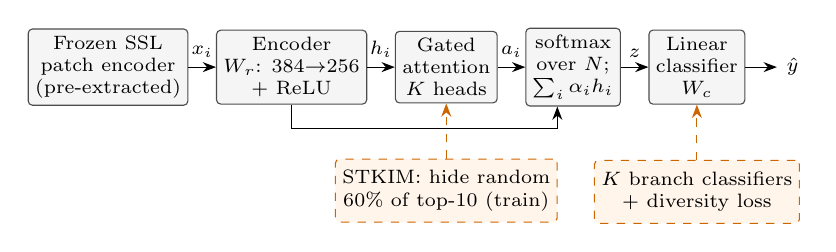
\begin{tikzpicture}[>=Stealth, node distance=4mm and 3.5mm,
  every node/.style={font=\scriptsize},
  box/.style={draw=black!70, rounded corners=1.5pt, align=center, minimum height=8mm, inner sep=2.5pt, fill=black!4},
  ext/.style={box, draw=orange!80!black, fill=orange!8, dashed}]
\node[box] (enc) {Frozen SSL\\patch encoder\\(pre-extracted)};
\node[box, right=of enc] (red) {Encoder\\$W_r$: 384$\to$256\\+ ReLU};
\node[box, right=of red] (att) {Gated\\attention\\$K$ heads};
\node[box, right=of att] (pool) {softmax\\over $N$;\\$\sum_i\alpha_i h_i$};
\node[box, right=of pool] (cls) {Linear\\classifier\\$W_c$};
\draw[->] (enc) -- node[above]{$x_i$} (red);
\draw[->] (red) -- node[above]{$h_i$} (att);
\draw[->] (att) -- node[above]{$a_i$} (pool);
\draw[->] (pool) -- node[above]{$z$} (cls);
\draw[->] (cls.east) -- ++(4mm,0) node[right]{$\hat y$};
\draw[->] (red.south) -- ++(0,-3mm) -| ([xshift=-2mm]pool.south);
\node[ext, below=7mm of att] (mask) {STKIM: hide random\\60\% of top-10 (train)};
\node[ext, below=7mm of cls] (br) {$K$ branch classifiers\\+ diversity loss};
\draw[->, orange!80!black, dashed] (mask.north) -- (att.south);
\draw[->, orange!80!black, dashed] (br.north) -- (cls.south);
\end{tikzpicture}}
\caption{ABMIL pipeline (grey; $K{=}1$) and the additions of the implemented extension (orange, dashed; $K{=}5$). Only the grey modules after the frozen encoder are trained in the baseline.}
\label{fig:arch}
\end{figure}

\subsection{Training and evaluation protocol}
We use the provided configuration: AdamW~\cite{loshchilov2019adamw} with learning rate $10^{-4}$ and weight decay $10^{-5}$, cross-entropy loss, $B{=}1$, no dropout, 30 epochs and a constant learning rate. Each epoch visits every training slide once in a new random order (only the training loader shuffles). After every epoch the model is evaluated on the validation set, and the checkpoint with the highest validation macro-AUC $+$ macro-F1 is kept; this checkpoint is evaluated once on the test set. We report test macro-AUC, accuracy and macro-F1 (torchmetrics, one-vs-rest macro AUC). Each configuration is run with five training seeds (0--4), which change the initialisation and the shuffling order but not the data split; we report mean $\pm$ standard deviation. All runs used one NVIDIA Tesla T4 GPU (Google Colab) with PyTorch 2.11 (CUDA 13.0). The features of each dataset are cached once on the GPU as float16, identically for all methods; a 30-epoch run then takes 15--85\,s (40\,s on average for ABMIL, 70\,s for the extension), and all 90 runs take 64 GPU-minutes.

\subsection{Observations on model structure and training}\label{sec:observations}
\emph{Small model on large bags.} The trainable part is a shallow network of $\approx$165k parameters, while a bag holds thousands of 384-d vectors. Cost and memory are linear in $N$, so a whole slide fits in one forward pass and a full 30-epoch run on cached features takes well under two minutes on a T4 GPU. The capacity sits almost entirely in the encoder $W_r$ and the attention scorer; the slide classifier is linear.

\emph{Few, noisy updates.} With $B{=}1$ there are only a few hundred optimisation steps per epoch, each computed from one slide, so gradients are noisy and the class balance of an update depends on the shuffling order. There is no normalisation layer and no learning-rate schedule: the \texttt{warmup\_epoch} entry in the configuration is not used by the provided loop.

\emph{The attention is the only instance selection.} Every patch contributes to $z$ through $\alpha_i$, so the softmax decides which tissue the classifier sees. Because $\alpha$ is shared by all classes, a single distribution must serve, e.g., both the evidence for ``tumour'' and the evidence for ``normal''.

\emph{Model selection is noisy.} The validation sets contain only tens of slides (Table~\ref{tab:splits}), so validation AUC moves in coarse steps and can saturate; the selection rule keeps the \emph{first} epoch that reaches the maximum. We therefore also report the selected epoch and the spread across seeds.

\emph{Dataset-specific difficulty.} CAMELYON16 is binary but has small lesions (low witness rate); CAMELYON17 adds a centre shift between training and test and a four-class label in which ITC versus micro-metastasis depends on lesion size; BRACS has seven fine-grained classes with as few as 24 training slides per class, so macro-F1 is dominated by the hardest classes.

% =============================================================================
\section{Baseline Results}\label{sec:baseline-results}

\inputorpending{tables/baseline.tex}{ABMIL baseline results.}{tab:baseline}
\figureorpending{figures/loss_curves.pdf}{Learning curves (mean $\pm$ std over five seeds). Solid: ABMIL training loss; dashed: validation cross-entropy of ABMIL (blue) and of the extension (orange). Validation loss is the plain slide-level cross-entropy for both models and is directly comparable.}{fig:loss}

Table~\ref{tab:baseline} gives the baseline and Fig.~\ref{fig:loss} its learning curves.

\emph{Performance.} ABMIL reaches a test macro-AUC of $0.914\pm0.034$ on CAMELYON16, $0.855\pm0.012$ on CAMELYON17 and $0.807\pm0.010$ on BRACS. Macro-F1 orders the datasets the same way but separates them much more (0.869, 0.536 and 0.340), because it weights the rare and fine-grained classes equally. The seed-to-seed spread is largest on CAMELYON16, the easiest task, which points to model selection rather than to the model (see below).

\emph{Learning curves.} On CAMELYON17 and BRACS the curves show classic overfitting (Fig.~\ref{fig:loss}). The training loss falls monotonically to 0.04 and 0.12 (98.7\% and 96.6\% training accuracy at epoch 30), whereas the mean validation loss reaches its minimum at epoch 5 (0.455) and epoch 4 (1.388) and then rises to 0.764 and 2.617. Validation AUC peaks at about the same time (0.884 at epoch 5; 0.831 at epoch 7) and decays afterwards. The selection rule therefore stops early, at epochs 6--8 on BRACS and 11--18 on CAMELYON17, where macro-F1 is still improving after the AUC peak. On CAMELYON16 both losses approach zero and the validation AUC is exactly 1.000 from epoch 2 or 3 in every seed: the 27 validation slides are separated perfectly almost immediately, so the rule always selects one of the first three epochs and cannot distinguish good from bad checkpoints. The test AUC of these checkpoints still varies by $\pm0.034$, the main source of uncertainty on this dataset. The single notebook run with the configuration seed behaves the same way (selected epoch 3, test AUC 0.928).

\emph{Validation--test gap.} Validation AUC exceeds test AUC on every dataset (1.000 vs.\ 0.914, 0.879 vs.\ 0.855, 0.831 vs.\ 0.807). On CAMELYON17 part of the gap is expected, because the validation slides come from the training centres and the test slides from the two held-out centres.

\emph{Which classes fail.} Table~\ref{tab:perclass} gives per-class F1 computed from the test predictions of all five seeds. On CAMELYON16 the errors are mostly missed metastases: 97\% of the normal but only 74\% of the tumour slides are recognised. On CAMELYON17 the negative and macro-metastasis classes are learned (F1 0.89 and 0.81) but ITC and micro-metastasis are not (0.16 and 0.30): most ITC slides are called negative and more than half of the micro-metastases are called macro. The model detects tumour but cannot judge its extent, which is exactly what separates these classes, and only 18 ITC and 37 micro-metastasis slides are available for training. On BRACS only invasive carcinoma is recognised reliably (F1 0.83); the atypical classes FEA and ADH are the hardest (0.09 and 0.18), and the errors fall mostly on neighbouring classes of the benign-to-malignant spectrum (FEA is mostly predicted as PB or UDH, ADH as DCIS). With 43\% accuracy but 0.81 macro-AUC, the model ranks slides along that spectrum reasonably but draws poor boundaries between adjacent classes. Accuracy alone would be misleading on CAMELYON17, where it is dominated by the 121 negative test slides.

\begin{table*}[t]
\centering
\caption{Per-class test F1, computed from the pooled test predictions of the five seeds. Classes: CAMELYON16 normal (N) / tumour (T); CAMELYON17 negative / ITC / micro- / macro-metastasis; BRACS N / PB / UDH / FEA / ADH / DCIS / IC.}
\label{tab:perclass}
\setlength{\tabcolsep}{3.5pt}
\resizebox{\textwidth}{!}{%
\begin{tabular}{l cc cccc ccccccc}
\toprule
 & \multicolumn{2}{c}{CAMELYON16} & \multicolumn{4}{c}{CAMELYON17} & \multicolumn{7}{c}{BRACS} \\
\cmidrule(lr){2-3} \cmidrule(lr){4-7} \cmidrule(lr){8-14}
Method & N & T & Neg & ITC & Micro & Macro & N & PB & UDH & FEA & ADH & DCIS & IC \\
\midrule
ABMIL (baseline)    & 0.912 & 0.828 & 0.889 & 0.162 & 0.300 & 0.807 & 0.286 & 0.417 & 0.171 & 0.092 & 0.175 & 0.471 & 0.829 \\
Mean pooling        & 0.773 & 0.444 & 0.800 & 0.235 & 0.000 & 0.828 & 0.182 & 0.267 & 0.242 & 0.123 & 0.020 & 0.058 & 0.864 \\
Max pooling         & 0.912 & 0.822 & 0.923 & 0.047 & 0.383 & 0.878 & 0.500 & 0.371 & 0.169 & 0.057 & 0.141 & 0.298 & 0.893 \\
ACMIL (MBA + STKIM) & 0.885 & 0.813 & 0.845 & 0.286 & 0.424 & 0.900 & 0.421 & 0.383 & 0.226 & 0.176 & 0.176 & 0.490 & 0.887 \\
MBA only            & 0.896 & 0.810 & 0.912 & 0.307 & 0.462 & 0.899 & 0.484 & 0.367 & 0.231 & 0.159 & 0.344 & 0.372 & 0.933 \\
\bottomrule
\end{tabular}}
\end{table*}

\subsection{What each component contributes}\label{sec:components}
\emph{Encoder.} The frozen self-supervised encoder turns each tissue patch into a 384-d morphological descriptor; it determines what can be distinguished at all (cell density, nuclear atypia, gland structure) and was learned without labels. The trainable projection $W_r$ with ReLU (Eq.~\ref{eq:enc}) adapts these generic descriptors to the task and to the attention module, compresses them to 256 dimensions, and is shared by every patch, so it acts as a learned instance-level feature selector.

\emph{Aggregator.} The gated attention (Eqs.~\ref{eq:att}--\ref{eq:pool}) scores each patch from its own embedding and pools the bag into a single vector $z$ that is a convex combination of the instance embeddings. It is what makes the model permutation-invariant and able to handle any $N$, and it decides how much of the slide the classifier sees: it can emulate max pooling (one patch with $\alpha_i\approx1$) or mean pooling (uniform $\alpha$). Its weights provide the attention maps used for interpretation (Fig.~\ref{fig:wsi}).

\emph{Classifier.} The linear head (Eq.~\ref{eq:cls}) maps the slide embedding to class logits. Because both the pooling and the head are linear in $h_i$, the logit of class $c$ decomposes exactly into patch contributions,
\begin{equation}
\hat y_c=\sum_{i=1}^{N}\alpha_i\,\big(w_{c}^\top h_i\big)+b_c, \label{eq:additive}
\end{equation}
so a patch matters through the product of \emph{how much it is attended} and \emph{what it says about class $c$}. The attention alone is therefore an incomplete explanation (it is unsigned and class-agnostic); we build on this in Proposal~2.

\inputorpending{tables/aggregator.tex}{Aggregator ablation.}{tab:aggregator}

Table~\ref{tab:aggregator} quantifies the aggregator's contribution by replacing attention with mean or max pooling while keeping the same encoder, classifier and training protocol.
Learned attention is far better than mean pooling on every dataset ($\Delta$AUC $-0.277$, $-0.057$ and $-0.146$ for mean pooling, worse on all seeds, $p\le0.008$ in a paired t-test). The drop is largest on CAMELYON16, where mean pooling recognises only 83 of 245 tumour slides over five seeds: averaging over about 12{,}500 patches per slide dilutes a lesion that covers a small fraction of the tissue, the failure expected when the witness rate is low (Sec.~\ref{sec:lit}). Mean pooling also underfits (82\% and 71\% training accuracy after 30 epochs on CAMELYON16 and BRACS), because the average embeddings of different classes are too similar. Max pooling behaves differently. On the lymph-node datasets it is \emph{better} than attention (CAMELYON16 $0.944\pm0.009$, $+0.030$ on 4/5 seeds; CAMELYON17 $0.874\pm0.006$, $+0.019$ on 5/5 seeds) and has the smallest seed-to-seed spread, but on BRACS it is clearly worse ($0.765$, $-0.042$ on all seeds). This matches the pooling assumptions: metastasis detection follows the standard MIL assumption (a few tumour patches make a slide positive), which max pooling encodes directly, whereas BRACS subtypes are defined by the architecture of larger regions and by the absence of atypia, which a feature-wise maximum over single patches cannot represent. Attention lies between the two and is the only aggregator that is competitive on all three tasks, but it is not the best choice for every task, and its flexibility costs variance on CAMELYON16. Macro-F1 does not separate max pooling and attention on CAMELYON16 and BRACS, and max pooling almost never predicts ITC (F1 0.05, Table~\ref{tab:perclass}).

\begin{figure}[t]
\centering
\IfFileExists{figures/wsi_attention_test_068.png}{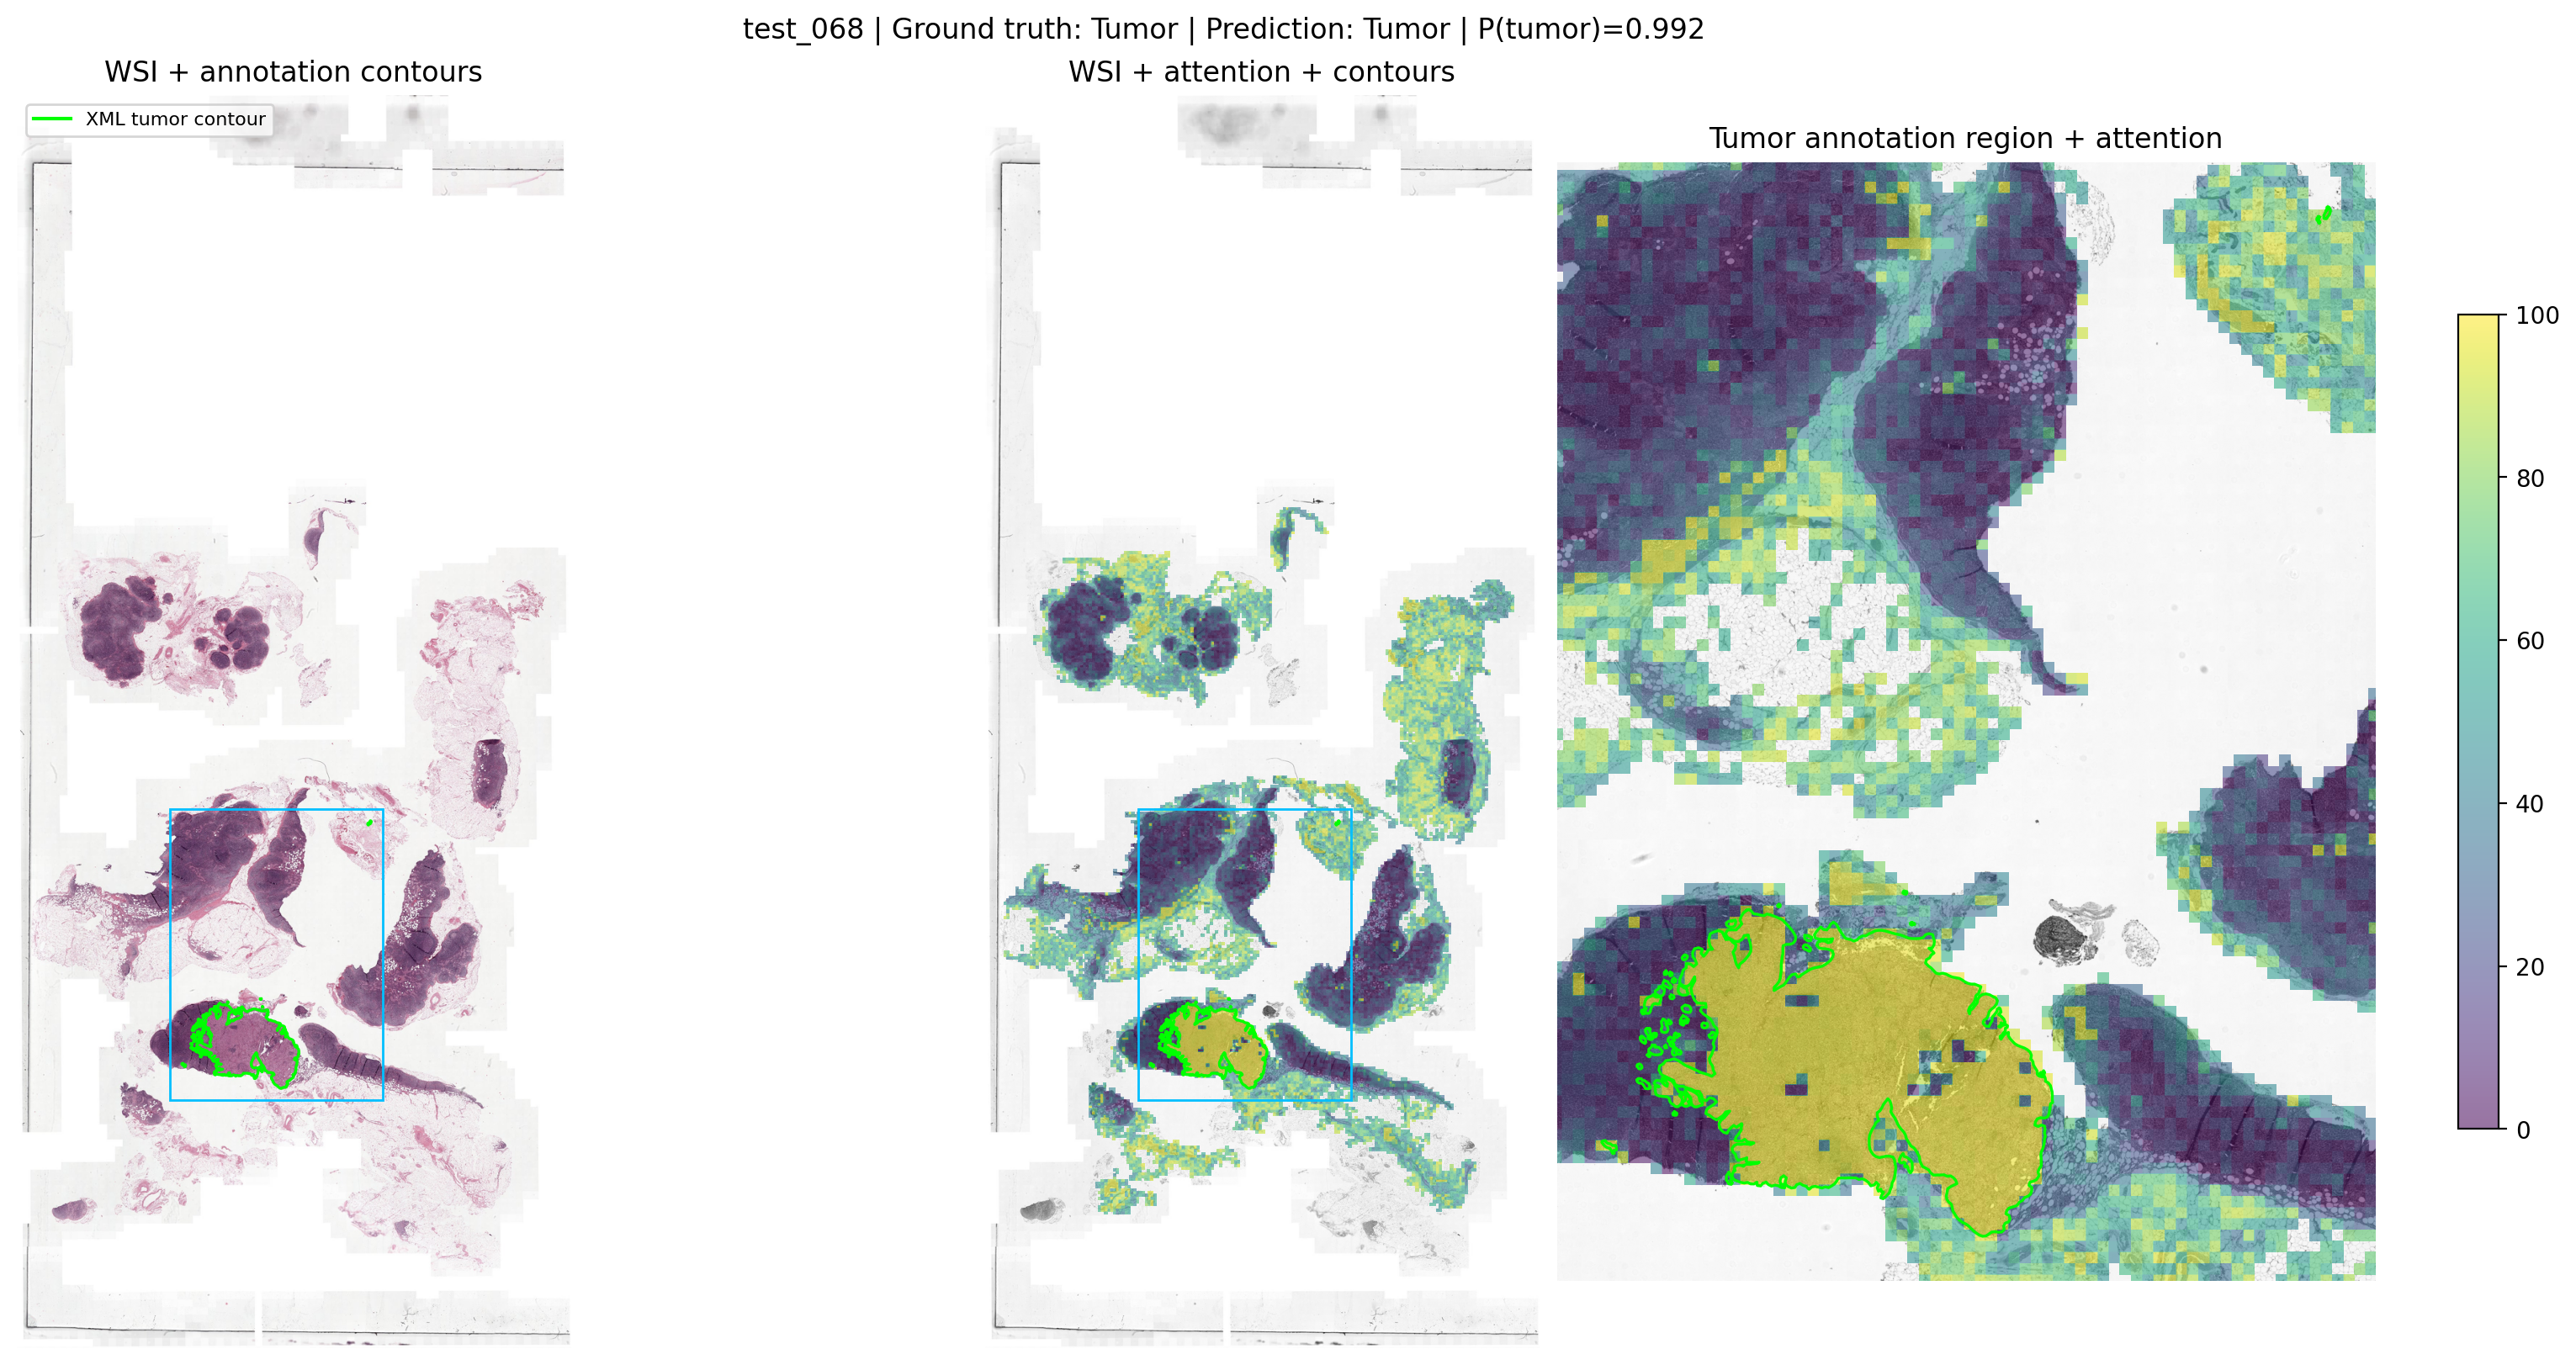
\includegraphics[width=\columnwidth]{figures/wsi_attention_test_068.png}\\[-1mm]{\footnotesize (a) ABMIL}\\[1mm]}{%
\fbox{\parbox{0.9\columnwidth}{\centering\small Run the notebook with \texttt{DATASET='C16'}: Step 8 saves\\ \texttt{report/figures/wsi\_attention\_test\_068.png}.}}\\[1mm]}
\IfFileExists{figures/wsi_attention_acmil_test_068.png}{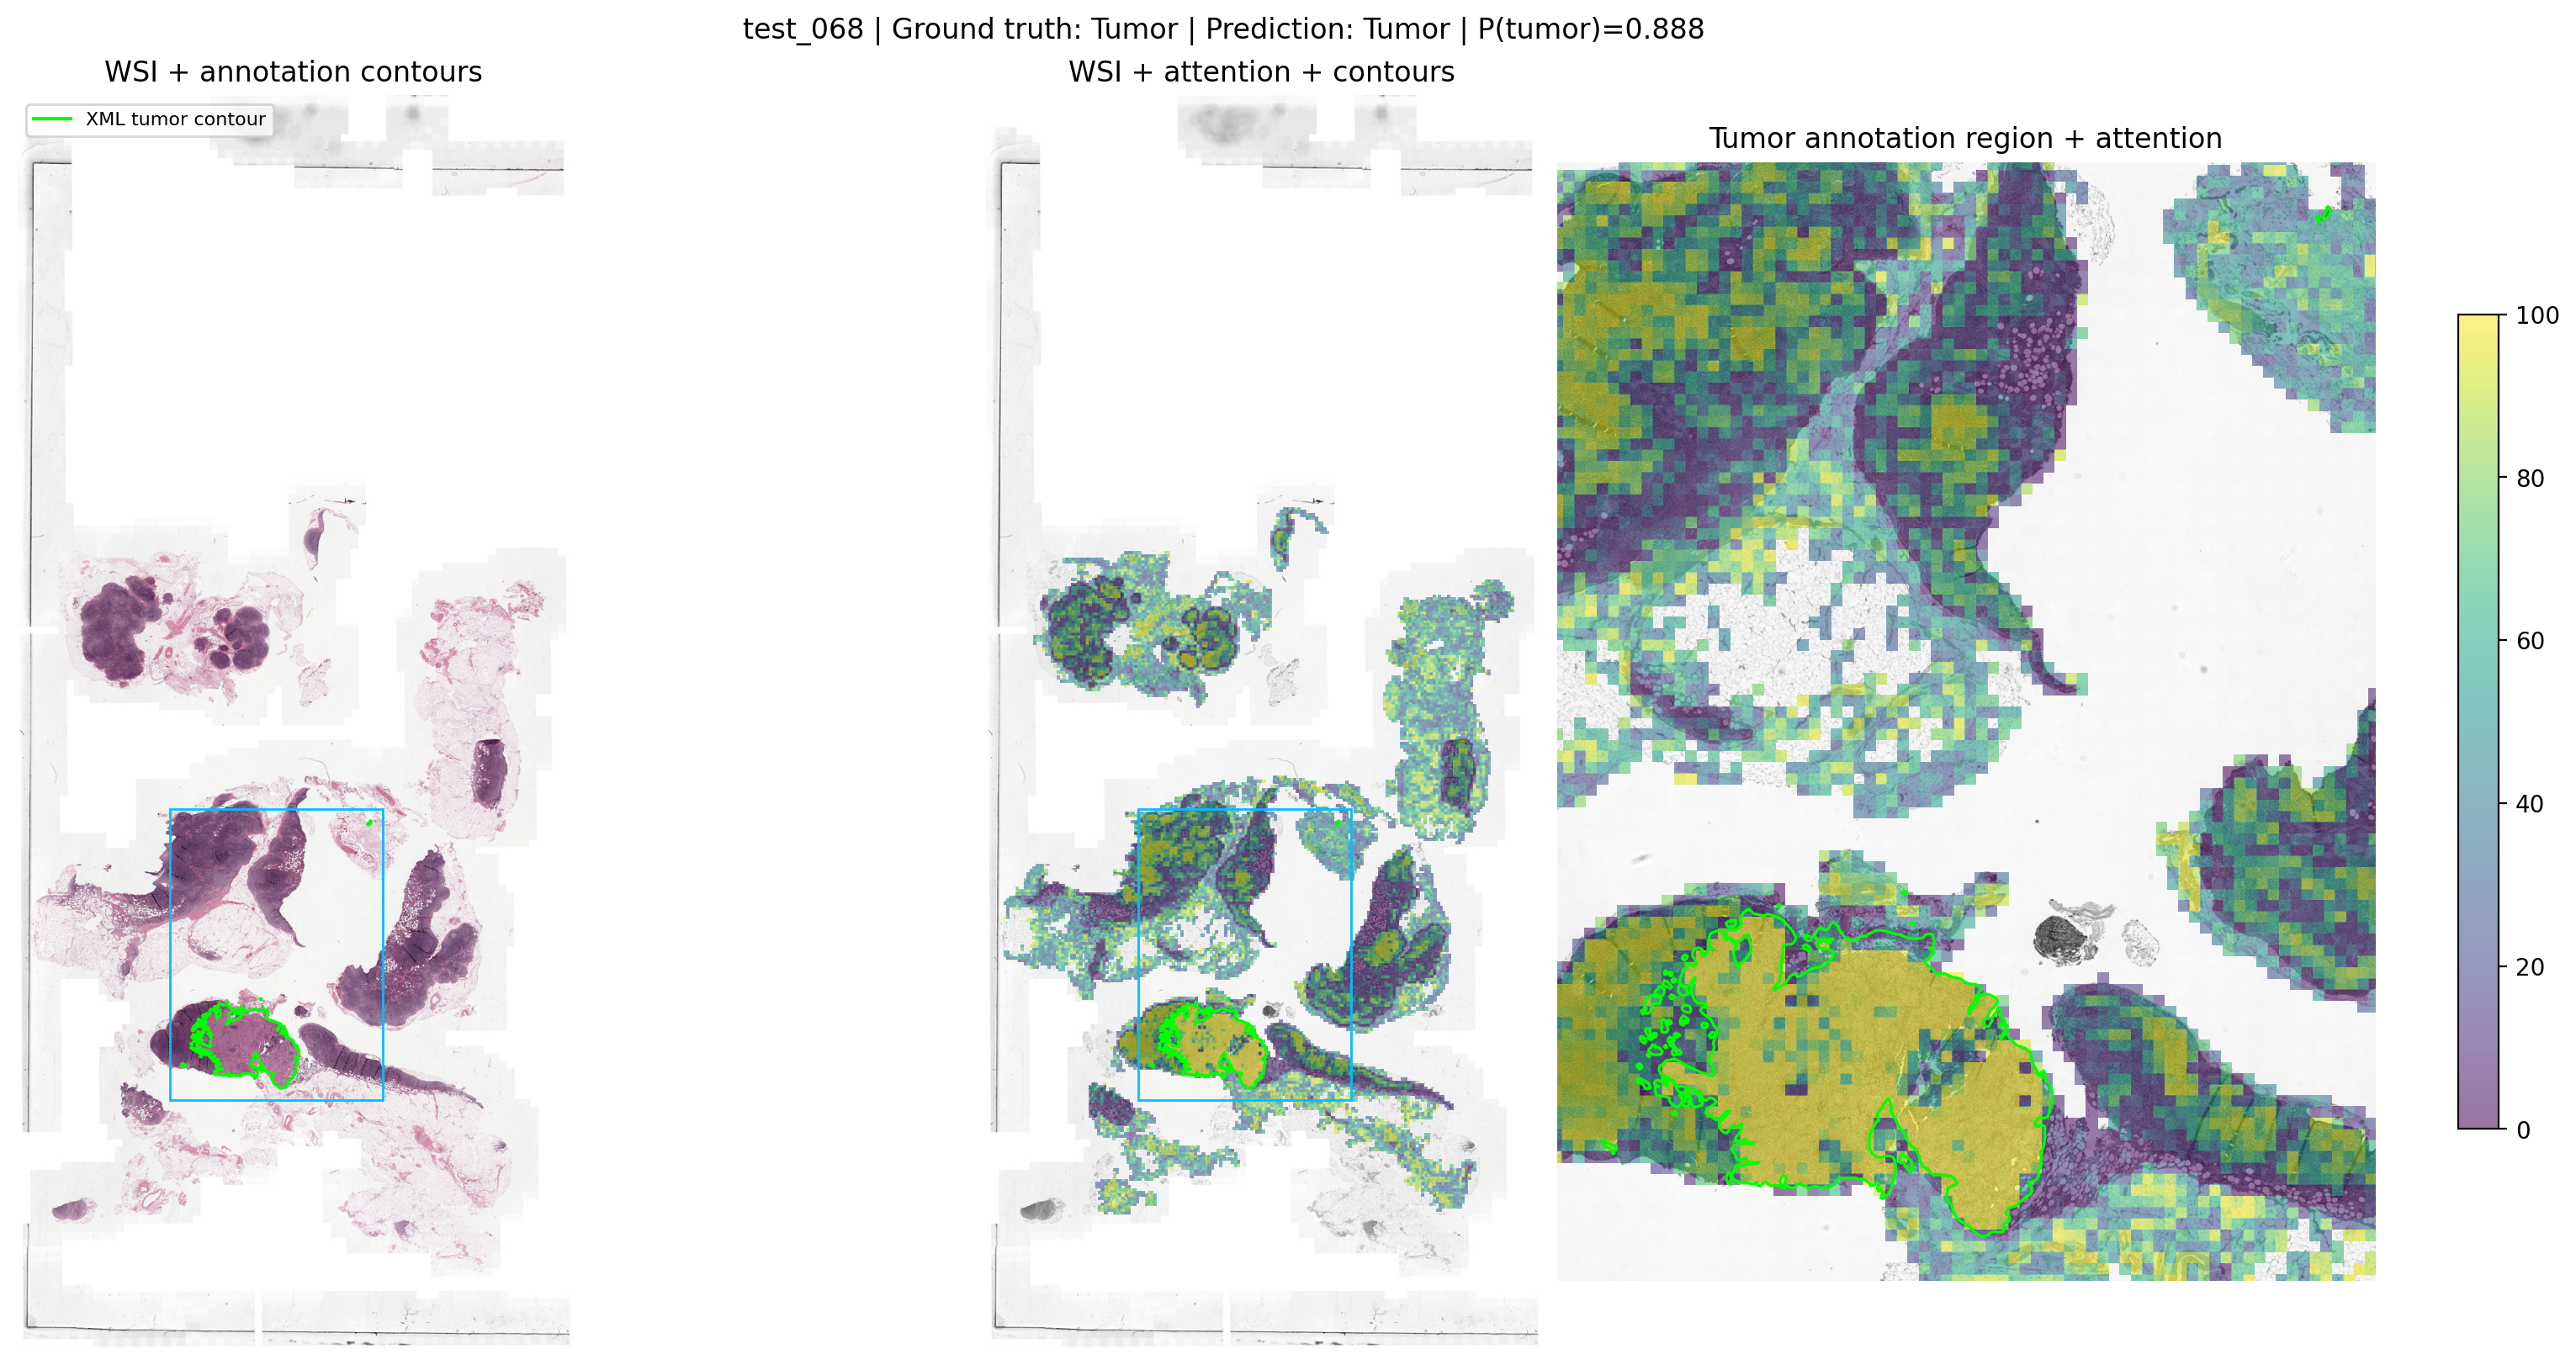
\includegraphics[width=\columnwidth]{figures/wsi_attention_acmil_test_068.png}\\[-1mm]{\footnotesize (b) Extension (ACMIL)}}{}
\caption{Attention on CAMELYON16 \texttt{test\_068} (tumour) with the annotated tumour contour (green) for (a) ABMIL and (b) the extension (Step 9 of the notebook). Colours are within-slide attention percentiles, not tumour probabilities.}
\label{fig:wsi}
\end{figure}
On the tumour slide \texttt{test\_068} (Fig.~\ref{fig:wsi}a; notebook run, $P(\text{tumour})=0.992$) the highest-percentile ABMIL attention covers the annotated metastasis almost completely, with additional high attention at a few tissue borders. On the normal slide \texttt{test\_067} ($P=0.029$) the highest attention lies on the capsule and tissue edges, and there is no single focus. Over all test slides, ABMIL attention on CAMELYON16 tumour slides is concentrated (normalised entropy 0.66, 52\% of the mass on the top 1\% of patches) and nearly uniform on normal slides (0.96 and 11\%). The extension (Fig.~\ref{fig:wsi}b, $P=0.888$) still ranks the tumour highest but spreads high attention over much more of the surrounding lymphoid tissue; Sec.~\ref{sec:extension} shows what this does to the predictions.

% =============================================================================
\section{Research Proposals}\label{sec:proposals}

\subsection{Proposal 1 (implemented): attention-challenging MIL}\label{sec:p1}
\emph{Motivation.} With a few hundred training slides, ABMIL can reach near-zero training loss by placing almost all attention mass on a few extremely discriminative patches of each training slide. This attention over-concentration~\cite{zhang2024acmil} has two costs: the model learns a narrow set of patterns that may not recur in new slides (or in new centres, as in CAMELYON17), and the remaining evidence in the slide receives almost no gradient through $\alpha$. We expect the problem to be strongest on CAMELYON16/17, where tumour regions are small, and when the number of training slides is small.

\emph{Design.} We keep the baseline encoder and gated scorer and change only the aggregation and the objective (Fig.~\ref{fig:arch}, orange):
\begin{enumerate}
\item \textbf{Multi-branch attention (MBA).} The scorer outputs $K{=}5$ attention logits per patch, $a^{(k)}_i$, giving $K$ attention distributions $\alpha^{(k)}$ and branch embeddings $z_k=\sum_i\alpha^{(k)}_i h_i$, each with its own linear classifier $\hat y_k$. A diversity term penalises the mean pairwise cosine similarity of the branches' attention vectors, $\mathcal{L}_{\text{div}}=\frac{2}{K(K-1)}\sum_{k<l}\cos(\alpha^{(k)},\alpha^{(l)})$, so the branches are pushed to base their (correct) predictions on different patches.
\item \textbf{Stochastic top-$k$ instance masking (STKIM).} During training only, for every branch we find its $m{=}10$ highest-scoring patches and set the logits of a random 60\% of them to $-\infty$ before the softmax. The model must therefore also learn from patches that are not its current favourites.
\item \textbf{Slide prediction.} The final prediction $\hat y$ comes from a separate linear classifier applied to $\bar z=\sum_i\bar\alpha_i h_i$ with the branch-averaged attention $\bar\alpha=\frac1K\sum_k\alpha^{(k)}$.
\end{enumerate}
The training objective is
\begin{equation}
\mathcal{L}=\CE(\hat y,Y)+\frac1K\sum_{k=1}^{K}\CE(\hat y_k,Y)+\lambda\,\mathcal{L}_{\text{div}},\qquad \lambda=1.
\end{equation}
At test time masking is off, so inference is deterministic and costs the same as ABMIL up to the $K$ scorer outputs; the model has 167{,}825, 170{,}909 and 175{,}535 parameters on the three datasets, 2--6\% more than ABMIL.

\emph{Rationale for the design choices.} (i) Masking targets the \emph{top-attended} patches rather than random patches because a random 1\% instance dropout on a bag of $10^4$ patches would almost never remove the few patches that carry all the attention; (ii) only a random subset of the top patches is hidden, so the model is challenged but still sees some of the strongest evidence and the slide label remains supported; (iii) masking is applied to logits before the softmax, so the remaining weights still sum to one; (iv) several branches with a diversity penalty are a cheap way to cover several distinct regions of a slide without the parameters of a transformer, and each branch has its own classifier so that every branch must be predictive on its own; (v) averaging the branch attentions for the final prediction pools the evidence of all branches into one embedding; (vi) we keep all optimisation hyper-parameters identical to the baseline and adopt $K{=}5$, $m{=}10$, 60\% masking and $\lambda{=}1$ from~\cite{zhang2024acmil} without tuning, so that any difference is attributable to the method rather than to extra tuning on our small validation sets.

\emph{Hypotheses.} \textbf{H1}: the attention of the extension is less concentrated than ABMIL's (higher normalised entropy, lower mass on the top 1\% of patches). \textbf{H2}: test AUC and macro-F1 improve, most on the datasets with small lesions. \textbf{H3}: MBA and STKIM are complementary, i.e.\ each alone helps less than both.

\subsection{Proposal 2 (not implemented): faithful, class-specific patch attributions}\label{sec:p2}
\emph{Motivation.} ABMIL heatmaps show $\alpha_i$, which is unsigned and shared across classes: a patch can be highly attended because it is strong evidence \emph{against} the predicted class. Clinicians need to know which tissue supports which diagnosis, and attention is known to be an unreliable explanation in general~\cite{jain2019attention}.

\emph{Design.} Eq.~\eqref{eq:additive} shows that, for the baseline, the exact contribution of patch $i$ to class $c$ is $\phi_{i,c}=\alpha_i\,w_c^\top h_i$ (and $\phi_{i,c}-\phi_{i,c'}$ for a two-class decision), available at no extra cost. For heads that are not linear (e.g.\ an MLP classifier or TransMIL), Additive MIL~\cite{javed2022additive} restores this property by applying the classifier per instance before pooling. We would compare four patch-importance maps for the same trained models: raw attention $\alpha_i$, the signed contribution $\phi_{i,\hat c}$, integrated gradients~\cite{sundararajan2017ig} with respect to $x_i$, and an Additive-MIL model trained with an MLP head.

\emph{Evaluation.} Explanation quality needs its own measurements: (a) \emph{faithfulness}, via deletion and insertion curves~\cite{samek2017evaluating,petsiuk2018rise}, i.e.\ removing (adding) patches in order of importance and measuring the area under the predicted-probability curve, on all three datasets; (b) \emph{localisation} on CAMELYON16, as the AUC of each patch-importance map for discriminating patches inside vs.\ outside the annotated tumour region; (c) \emph{sanity checks}~\cite{adebayo2018sanity}: the maps must change when the model weights are randomised; and (d) classification metrics, to verify that the Additive-MIL variant does not lose accuracy.

\emph{Why we implemented Proposal 1 first.} Proposal~2 needs patch-level tumour annotations for its localisation test, but the course package provides only one annotated slide (\texttt{test\_068}), so a convincing evaluation would be limited to deletion curves. Proposal~1 targets a problem we can measure on all three datasets with the available labels.

% =============================================================================
\section{Extension: Experiments and Results}\label{sec:extension}

\subsection{Setup}
The extension (``ACMIL'') and two ablations, \emph{MBA only} (5 branches and diversity loss, no masking) and \emph{STKIM only} (a single branch with masking), are trained with exactly the baseline protocol: same features, splits, optimiser, learning rate, epochs, selection rule and five seeds. Seeds are paired across methods, so we also report the per-seed difference to ABMIL. To test H1 we compute, for each test slide, the normalised attention entropy $\tilde H=-\sum_i\alpha_i\log\alpha_i/\log N\in[0,1]$ and the attention mass on the top 1\% of patches, and average over slides.

\inputorpending{tables/extension.tex}{Extension vs.\ baseline and ablations.}{tab:extension}
\inputorpending{tables/attention.tex}{Attention concentration.}{tab:attention}
\figureorpending{figures/val_auc_curves.pdf}{Validation macro-AUC per epoch (mean $\pm$ std over five seeds) for ABMIL, the extension and its ablations.}{fig:valauc}
\begin{figure}[t]
\centering
\IfFileExists{figures/attention_entropy.pdf}{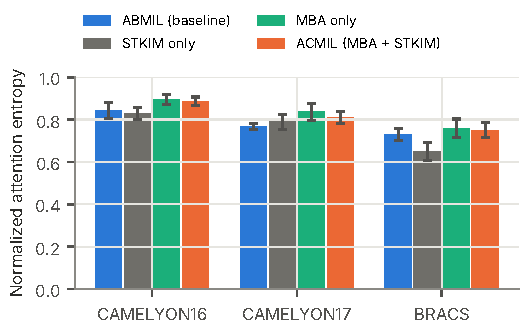
\includegraphics[width=0.9\columnwidth]{figures/attention_entropy.pdf}}{\fbox{\parbox{0.8\columnwidth}{\centering\small Generated by \texttt{summarize\_results.py}.}}}
\caption{Normalised attention entropy on the test slides (mean $\pm$ std over five seeds); 1 is uniform attention.}
\label{fig:attn}
\end{figure}

\subsection{Results}
\emph{H2 (classification).} On CAMELYON17 the extension improves macro-AUC on every seed ($0.872\pm0.006$ vs.\ $0.855\pm0.012$; paired $\Delta=+0.017\pm0.015$) and macro-F1 by $+0.077$ (5/5 seeds, $p=0.03$), with the largest per-class gains on the rare ITC and micro-metastasis classes (F1 0.16$\to$0.29 and 0.30$\to$0.42, Table~\ref{tab:perclass}). Accuracy does not improve ($75.7\pm7.7$\% vs.\ $77.2\pm3.5$\%), because more negative slides are now called ITC. On BRACS macro-AUC is unchanged within noise ($+0.005\pm0.023$, 3/5 seeds), while macro-F1 rises from 0.340 to 0.382 (4/5 seeds, $p=0.06$), mainly on the normal, FEA and invasive-carcinoma classes. On CAMELYON16 the extension is not better: $+0.004\pm0.056$ AUC (3/5 seeds) and lower accuracy and macro-F1. It finds more metastases (200 vs.\ 181 of 245 tumour slides over five seeds) but produces four times as many false positives (47 vs.\ 11 of 400 normal slides). The differences on CAMELYON16 and in BRACS AUC lie well inside the seed-to-seed standard deviation and should be read neither as improvements nor as degradations.

\emph{H1 (attention concentration).} The extension raises the normalised attention entropy on all three datasets (0.84$\to$0.89, 0.77$\to$0.81, 0.73$\to$0.75; Table~\ref{tab:attention}, Fig.~\ref{fig:attn}), but the mass on the top 1\% of patches falls only on CAMELYON16 (0.26$\to$0.23) and is unchanged on the other two, so H1 holds only weakly. The change comes from the multiple branches: MBA alone gives the same or a higher entropy, whereas STKIM alone leaves CAMELYON16/17 unchanged and makes BRACS attention \emph{more} concentrated (entropy 0.65, top-1\% mass 0.57). When a single branch loses its favourite patches during training, it learns to rank similar neighbouring patches even higher instead of spreading out. Per class, the extension changes attention most where ABMIL is most concentrated: on CAMELYON16 tumour slides the top-1\% mass drops from 0.52 to 0.29, and on CAMELYON17 micro-metastasis slides from 0.87 to 0.61. These are slides with small lesions, so spreading attention is not necessarily desirable there, as the CAMELYON16 false positives show.

\emph{H3 (complementarity).} H3 is rejected. MBA alone is at least as good as the full extension everywhere. On CAMELYON17 it gives the best AUC of all attention models ($0.884\pm0.013$, $+0.029\pm0.005$ on 5/5 seeds, $p<0.001$), macro-F1 0.639 and 6 points more accuracy, and on BRACS the best macro-F1 (0.398, 5/5 seeds, $p=0.007$). STKIM alone is never better than ABMIL ($\Delta$AUC $-0.016$, $-0.007$ and $-0.003$), and adding it to MBA lowers the CAMELYON17 AUC.

\emph{Overfitting.} The learning curves show the mechanism behind the gains. On CAMELYON17 the validation loss of the extension stays flat after epoch 10 (minimum 0.402 at epoch 16, 0.414 at epoch 30), whereas ABMIL's rises from 0.455 to 0.764 (Fig.~\ref{fig:loss}); on BRACS the late rise is reduced from $+1.23$ to $+0.50$. The extension never fits the training set completely (95.5\% and 85.4\% training accuracy at epoch 30 on CAMELYON17 and BRACS), its validation AUC decays less late in training (Fig.~\ref{fig:valauc}), and its selected epochs move later (17--29 on CAMELYON17, 10--20 on BRACS). The extension therefore acts mainly as a regulariser, at about $1.7\times$ the training time (70\,s vs.\ 40\,s per run on average).

\subsection{Discussion}
Of the three hypotheses, H1 holds for entropy only, H2 holds on CAMELYON17 (AUC and macro-F1) and for BRACS macro-F1 but not on CAMELYON16, and H3 is rejected: the useful component is the multi-branch attention with its auxiliary branch losses, not the masking. We see five reasons for this pattern.
(i)~Where no effect is visible, model selection is the limiting factor. On CAMELYON16 every attention model reaches validation AUC 1.0 within five epochs, so the selected checkpoint is essentially the first one that separates 27 slides, and the paired seed-to-seed differences (standard deviation 0.03--0.08 AUC) are much larger than any difference between methods.
(ii)~On CAMELYON16 the over-concentration hypothesis does not fit the data. Concentrated attention is the right inductive bias for small metastases, as max pooling being the best aggregator there (0.944) shows, and spreading attention increases false positives.
(iii)~Where ABMIL clearly overfits (CAMELYON17 and BRACS, Fig.~\ref{fig:loss}), the regularisation helps, most on the rare classes that a single attention head fits from very few examples. This agrees with the motivation of~\cite{zhang2024acmil} that diverse branches use more of the available evidence.
(iv)~With the published setting, STKIM hides only 6 of roughly 10{,}000 patches per branch. Neighbouring patches have nearly identical features, so the model simply moves its attention to a neighbour; this explains why masking alone changes nothing or even sharpens attention. The hyper-parameters were adopted without tuning.
(v)~Attention regularisation addresses neither the centre shift of CAMELYON17 nor the fine-grained class boundaries of BRACS, which remain the dominant errors (Table~\ref{tab:perclass}).
The following experiments would discriminate between these explanations: a masking ratio proportional to the bag size (e.g.\ 1--5\% of the patches) to test (iv); training on fewer slides (\texttt{n\_shot}) to test whether the gain grows with data scarcity; an ablation with $\lambda=0$ that separates the diversity loss from the auxiliary branch losses; and repeated or cross-validated splits for CAMELYON16, so that model selection is not decided by 27 slides.

Limitations of our study: all models use one frozen feature extractor; results come from a single split per dataset (the seeds vary only the training randomness), and the validation sets are small. Attention statistics describe where the model looks, not whether that is clinically correct; Proposal~2 addresses that question.

% =============================================================================
\section{Conclusion}
We implemented ABMIL in PyTorch and evaluated it on three WSI benchmarks with a fixed, leakage-free protocol, explained the role of the encoder, attention aggregator and linear classifier, and showed with an aggregator ablation what learned attention adds over fixed pooling. We proposed two extensions and implemented an attention-challenging variant with multi-branch attention and stochastic top-$k$ masking. Attention is essential compared with mean pooling ($+0.06$ to $+0.28$ AUC) but not uniformly better than max pooling, which wins on the two lymph-node datasets. The extension improves CAMELYON17 consistently and macro-F1 on CAMELYON17 and BRACS by reducing overfitting, while its effect on CAMELYON16 is within noise, and the gain comes from the multiple attention branches rather than from top-$k$ masking. The most important lesson is methodological: with validation sets of 27--62 slides, model selection and seed variance are as large as the effects under study, so claims need several seeds and paired comparisons.

\bibliographystyle{IEEEtran}
\bibliography{refs}

\appendices
% =============================================================================
\section{Reproducibility checklist for this report}\label{app:checklist}
Following the ML reproducibility checklist~\cite{pineau2021reproducibility}. The code repository is a separate artefact with its own checklist in its \texttt{README.md}.

\smallskip\noindent\textbf{Models and algorithms.}
Mathematical description of the model and algorithm: yes, Secs.~\ref{sec:model} and~\ref{sec:p1}.
Assumptions: yes, frozen features (Sec.~\ref{sec:baseline}), split construction (Table~\ref{tab:splits}).
Complexity: parameter counts in Secs.~\ref{sec:model} and~\ref{sec:p1}; time and memory are linear in the number of patches; measured run times in \texttt{results/all\_runs.csv}.

\smallskip\noindent\textbf{Theoretical claims.} None beyond the exact decomposition in Eq.~\eqref{eq:additive}, which follows from linearity.

\smallskip\noindent\textbf{Datasets.}
Statistics and splits: Table~\ref{tab:splits}.
Excluded data: the provided HDF5 files contain 499 of the 500 CAMELYON17 training slides and 537 of the 547 BRACS slides; nothing else was removed.
Pre-processing: none beyond the provided feature extraction; features are cached on the GPU as float16.
Download: \url{https://zenodo.org/records/23130543}.

\smallskip\noindent\textbf{Code.} Dependencies (\texttt{requirements.txt}), training and evaluation code, trained checkpoints and per-run outputs, and the exact commands are in the repository README.

\smallskip\noindent\textbf{Experimental results.}
Hyper-parameters: all listed in Sec.~\ref{sec:baseline}; no hyper-parameter was tuned on the test set; the extension's hyper-parameters were taken from~\cite{zhang2024acmil}.
Number of runs: five training seeds per dataset and method, one evaluation of the selected checkpoint each.
Statistics: macro-AUC (one-vs-rest), accuracy, macro-F1; mean $\pm$ sample standard deviation over seeds; paired per-seed differences.
Run time and infrastructure: one NVIDIA Tesla T4 GPU (Google Colab, 2 vCPUs, 12.7\,GB RAM), PyTorch 2.11.0 with CUDA 13.0; 15--85\,s per 30-epoch run (per-run times in \texttt{results/all\_runs.csv}); 64 GPU-minutes for all 90 runs.

% =============================================================================
\section{Answers to the notebook questions}\label{app:answers}
\emph{Dataset vs.\ DataLoader.} A \texttt{Dataset} defines one sample (here a slide's bag of features, label and ID, read lazily from HDF5); a \texttt{DataLoader} defines how samples are served: order, batching via \texttt{collate\_fn} (padding plus mask), workers and pinned memory.
\emph{Shuffling.} Only the training loader shuffles, to decorrelate consecutive updates and avoid repeating the same ordering bias every epoch; evaluation metrics are order-independent and a fixed order keeps outputs aligned with IDs.
\emph{Shapes.} In $[B,N,D]$, $B$ is the number of slides per batch (1), $N$ the number of patches in the (padded) bag and $D{=}384$ the feature dimension.
\emph{Trainable tensors.} The weights of $W_r$, the attention $V,U,w$ (with biases) and the classifier $W_c,b_c$; features and attention weights are activations.
\emph{Softmax properties and alternatives.} Weights are positive, sum to one and are permutation-equivariant, so $z$ is a convex combination of the instances; alternatives include temperature-scaled softmax, sparsemax/entmax, normalised sigmoid gates, top-$k$/max or uniform weights.
\emph{\texttt{eval()} vs.\ \texttt{no\_grad()}.} \texttt{eval()} changes layer behaviour (dropout, batch-norm; and STKIM in our extension), \texttt{no\_grad()} stops autograd from recording the graph; evaluation needs both.
\emph{Omitting \texttt{zero\_grad()}.} Gradients would accumulate across steps, so every update would use the sum of all past gradients and training would become unstable.
\emph{Test set and model selection.} Selecting the epoch on test data fits the selection to test noise and biases the reported performance upwards; the test set must be used once after all decisions.

\end{document}
